常用的总线结构通常可分为\textbf{单总线结构、双总线结构和三总线结构。}

{\textbf{(1)单总线结构}}

\textbf{单总线结构是将CPU、主存、I/O设备(通过I/O接口)都连接在一组总线上,}允许I/O设备之间、I/O设备与CPU之间或I/O设备与主存之间直接交换信息,这种总线结构简单,很容易扩充外部设备,如下图所示。但是缺点也是显而易见的,所有的信息传送都通过这组共享总线,即不允许两个以上的部件在同一时刻向总线传输信息,这就必然会影响系统的工作效率。

所以,这类总线多\textbf{数被小型计算机或微型计算机采用}。另外,使用单总线结构肯定不能解决CPU、主存、I/O设备之间传输速率不匹配问题,故必须使用多总线结构。

\textbf{单总线的特点:}由于I/O设备与主存共用一组地址线,因此主存和I/O设备是统一编址的,CPU就可以像访问内存一样访问外部设备。

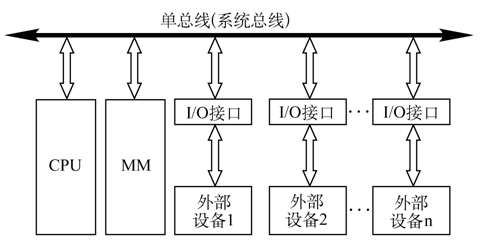
\includegraphics[width=6in]{png-jpeg-pics/9B4EDBB4E0AAF454E53B9A78F1B8AA1D.png}

{\textbf{(2)双总线结构}}\\

双总线的结构特点是\textbf{将速度较低的I/O设备从单总线中分离出来},形成主存总线与I/O总线分开的结构,如下图所示。\textbf{但双总线结构也有问题,}比如现在有三间房,主存住在最左边,CPU住在中间,I/O住在最右边,每次主存和I/O设备交换信息都要经过CPU,那CPU的工作效率就自然会降低,所以引进了三总线结构。

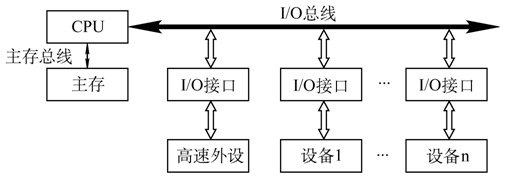
\includegraphics[width=6in]{png-jpeg-pics/33D71CE5A3125B7F5A4CD6D2D80FBD95.png}

{\textbf{(3)三总线结构}}

由下图可以看出,与双总线结构相比,三总线结构增加了一条小路(DMA总线),专门用于I/O高速设备与主存之间直接交换信息。DMA将在第7章的相关知识点讲解,这里只需知道这种结构即可。

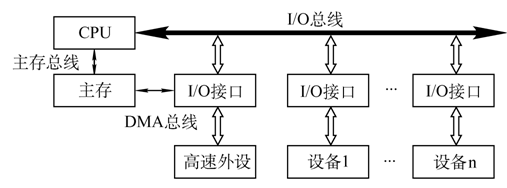
\includegraphics[width=6in]{png-jpeg-pics/FD242FF09C949861F0804447921171E8.png}
